\chapter{DORIS Ground Segment}
\label{ch:doris-ground-segment}

\tikzset{cross/.style={cross out, draw=red, minimum size=2*(#1-\pgflinewidth), inner sep=0pt, outer sep=0pt},
%default radius will be 1pt. 
cross/.default={1pt}}

\section{Geometry of Ground Antennae}
DORIS observations are referred to the electronic reference point (RP) of the antenna, 
the points where the DORIS observations  are  acquired.  As  that  electronic  point 
(\SI{2}{\GHz} center of phase for DORIS) is virtual and as for example it may change 
while using another type of antenna data referring to that electronic point are of no 
use for geophysical studies. So, observations must be referred to the conventional RP 
which is defined according to the geometry of the antenna. Therefore, one has also to 
account for the distance between the electronic RP and the conventional RP of the antenna (\cite{TOURAIN2016}). 
The ability to get accurate DORIS data relies for one part on the capability of providing 
accurate models to connect the  electronic RP (or electronic phase center) and the conventional 
RP, as well as, phase center variations (\gls{pcv}s) as a function of the elevation angle and azimuth.

The type of antenna is identified by the 4\textsubscript{th} character of the beacon 
mnemonic: letter ``A'' for the Alcatel type; letter ``B'' or letter ``C'' for the 
Starec B or C type.  That is, in the DORIS RINEX field ``STATION REFERENCE'', the 
last character of the second column (aka ``4-character station code''), defines the 
ground beacon antenna type; example:
\begin{verbatim}
    51                                                      # OF STATIONS       
D01  BEMB BELGRANO                      66018S002  3   0    STATION REFERENCE   
D02  ADHC TERRE ADELIE                  91501S005  3   0    STATION REFERENCE   
D03  SYQB SYOWA                         66006S005  3   0    STATION REFERENCE   
D04  CRQC CROZET                        91301S004  4   0    STATION REFERENCE   
D05  DIOB DIONYSOS                      12602S012  3   0    STATION REFERENCE
\end{verbatim}

\subsection{DORIS ALCATEL Antenna}


\begin{figure}
\centering
\begin{tikzpicture}
    \draw (2,-2) -- (2,-7); %% left vertical
    \coordinate (LT) at (2,-2);
    \draw (5,-2) -- (5,-7); %% right vertical
    \coordinate (RT) at (5,-2);
    \coordinate (L2PC) at (3.5, -4.0);
    \coordinate (L1PC) at (3.5, -3.0);
    \coordinate (BRP) at (3.5, -7.0);
    \draw (LT) to[out=60, in=120] (RT); %% dome
    \draw (LT) to (RT); %% top horizontal (under dome)
    \draw (1,-7) -- (6,-7); %% reference plain
    \draw (1, -7) -- (1, -7.5); %% left minor vertical
    \draw (6, -7) -- (6, -7.5); %% right minor vertical
    \draw [line width=0.25mm] (0,-7.5) -- (9,-7.5); %% ground
    \draw [-stealth] (3.5,-7.5) --node[anchor=west]{local vertical} (3.5, -8.5); %% local vertical to ground
    \draw [dotted] (3.5, 0) -- (3.5, -7.5); %% local vertical from dome
    
    \draw (L1PC) circle (2pt) node[anchor=south west]{phase center \SI{2}{\GHz}}; %% 2GHz pc
    \draw (L1PC) node[cross=3pt, rotate=0] {}; %% 2GHz cross
    \draw [dotted] (L1PC) -- (9.5, -3.0); %% horizontal from 2GHz PC
    \path (9.5, -7.0) -- node[](hl1){h\textsubscript{2GHz} = \SI{510}{\mm}} (9.5, -3.0);
    \draw [<-] (9.5, -7.0)--(hl1); \draw [->] (hl1)--(9.5, -3.0);
    
    \draw (L2PC) circle (2pt) node[anchor=south west]{phase center \SI{400}{\MHz}}; %% 400 MHz pc
    \draw (L2PC) node[cross=3pt, rotate=0] {}; %% 400MHz cross
    \draw [dotted] (L2PC) -- (9, -4.0); %% horizontal from 400MHz PC
    \path (8, -7.0) -- node[](hl2){h\textsubscript{400MHz} = \SI{335}{\mm}} (8, -4.0);
    \draw [<-] (8, -7.0)--(hl2); \draw[->] (hl2)--(8, -4.0);
    
    \draw (BRP) circle (2pt) node[anchor=south west]{DORIS reference point}; %% reference point
    \draw (BRP) node[cross=3pt, rotate=0] {}; %% RP cross
    \draw [dotted] (BRP) -- (10, -7.0); %% horizontal from RP
    \draw (10, -7) node[anchor=north west]{DORIS reference plane};
    
    \node[rectangle, align=left] (rptext) at (-1,-3.5) {DORIS reference point \\ \(\begin{bmatrix} x_s y_s z_s \end{bmatrix}^{T} \) beacon \\position in earth reference \\frame};
    \draw [-stealth] (rptext) to ($(BRP)-(3pt,-3pt)$);
    \node[above,font=\large\bfseries] at (current bounding box.north) {ALCATEL DORIS Ground Antenna};
\end{tikzpicture}
\caption{Geometry of Alcatel DORIS Ground Antenna/Beacon}
\label{fig:alcatel-antenna}
\end{figure}


\subsection{DORIS STAREC Antenna}
According to \cite{TOURAIN2016}, in order to check the consistency of the theoretical 
characteristics of this type of antennae, a measurement campaign was performedby 
the CNES at the Compact Antenna Test Range (CATR). The CATR is a dedicated facility 
consisting ofan anechoic chamber equipped with several specific devices 
allowing significant measurement for satellite characterization.

As a result of the campaign, a phase law was established by averaging the estimated 
phase law values obtained during the CATR characterization. The resulting couple phase 
center position–phase law correction was provided to the  DORIS  users  through  a  
text  file  in  \gls{antex} (\cite{ANTEXv14}) format, available on the IDS website
\url{ftp://ftp.ids-doris.org/pub/ids/stations/doris_phase_law_antex_starec.txt}.

STAREC antennae B and C are identical in terms of design and specification, the
difference is about the error budget in phase center position. For STAREC C,
manufacturing process and error budget have been improved (\cite{DORISGSM}).

\begin{figure}
\centering
\begin{tikzpicture}
    \coordinate (top) at (4,-1);
    \coordinate (tl) at (3.8, -1.3);
    \coordinate (tr) at (4.2, -1.3);
    \coordinate (blt) at (3.8, -3.0);
    \coordinate (brt) at (4.2, -3.0);
    \coordinate (blb) at (3.5, -3.3);
    \coordinate (brb) at (4.5, -3.3);
    \draw (top) to (tl);
    \draw (tl) to (blt);
    \draw (blt) to (blb);
    \draw (top) to (tr);
    \draw (tr) to (brt);
    \draw (brt) to (brb);
    \draw (blb) to (3.5, -9);
    \draw (brb) to (4.5, -9);
    \draw (3.5, -9) to (3.0, -9);
    \draw (3.0, -9) to (3.0, -9.3);
    \draw (4.5, -9) to (5.0, -9);
    \draw (5.0, -9) to (5.0, -9.3);
    \draw (3.0, -9.3) to (5.0, -9.3);

    \draw [dotted] (top) -- (4.0, -9.3); %% local vertical from top
    \draw [-stealth] (4.0, -9.3) -- node[anchor=west]{local vertical} (4.0, -10.3); %% local vertical arrow

    \coordinate (l1pc) at (4, -2.0);
    \draw (l1pc) circle (2pt) node[anchor=south west]{phase center \SI{2}{\GHz}}; %% 2GHz pc
    \draw (l1pc) node[cross=3pt, rotate=0] {}; %% 2GHz cross
    \draw (l1pc) to (10, -2.0);
    
    \coordinate (l2pc) at (4, -6.0);
    \draw [fill=black] (l2pc) circle (2pt) node[anchor=south west]{phase center \SI{400}{\MHz}}; %% 400MHz pc
    \draw (l2pc) node[cross=3pt, rotate=0] {}; %% 400MHz cross
    \draw ($(l2pc)-(1.0,0.0)$) -- node[below]{DORIS reference plane} (10, -6.0);
    \node (prt) at ($(l2pc)-(2.5,0.0)$) {Painted ring}; 
    \draw [-stealth] (prt) to ($(l2pc)-(0.2,0.0)$);

    \path ($(l1pc)+(5.5, 0.0)$) -- node[](h2g){h\textsubscript{2GHz} = \SI{487}{\mm}} ($(l2pc)+(5.5, 0.0)$);
    \draw [<-] ($(l1pc)+(5.5, 0.0)$) -- (h2g); \draw [->] (h2g) -- ($(l2pc)+(5.5, 0.0)$);

    \node[rectangle, align=left] (rptext) at ($(l2pc)-(2.0,2.0)$) {DORIS reference point \\ \(\begin{bmatrix} x_s y_s z_s \end{bmatrix}^{T} \) beacon \\position in earth reference \\frame};
    \draw [-stealth] (rptext) to ($(l2pc)-(3.5pt,4.5pt)$);

    \node[above,font=\large\bfseries] at (current bounding box.north) {STAREC DORIS Ground Antenna};
\end{tikzpicture}
\caption{Geometry of Alcatel STAREC Ground Antenna/Beacon}
\label{fig:alcatel-antenna}
\end{figure}

\section{Phase Law}

%\begin{figure}
%\begin{subfigure}{0.45\textwidth}
%  \centering
%  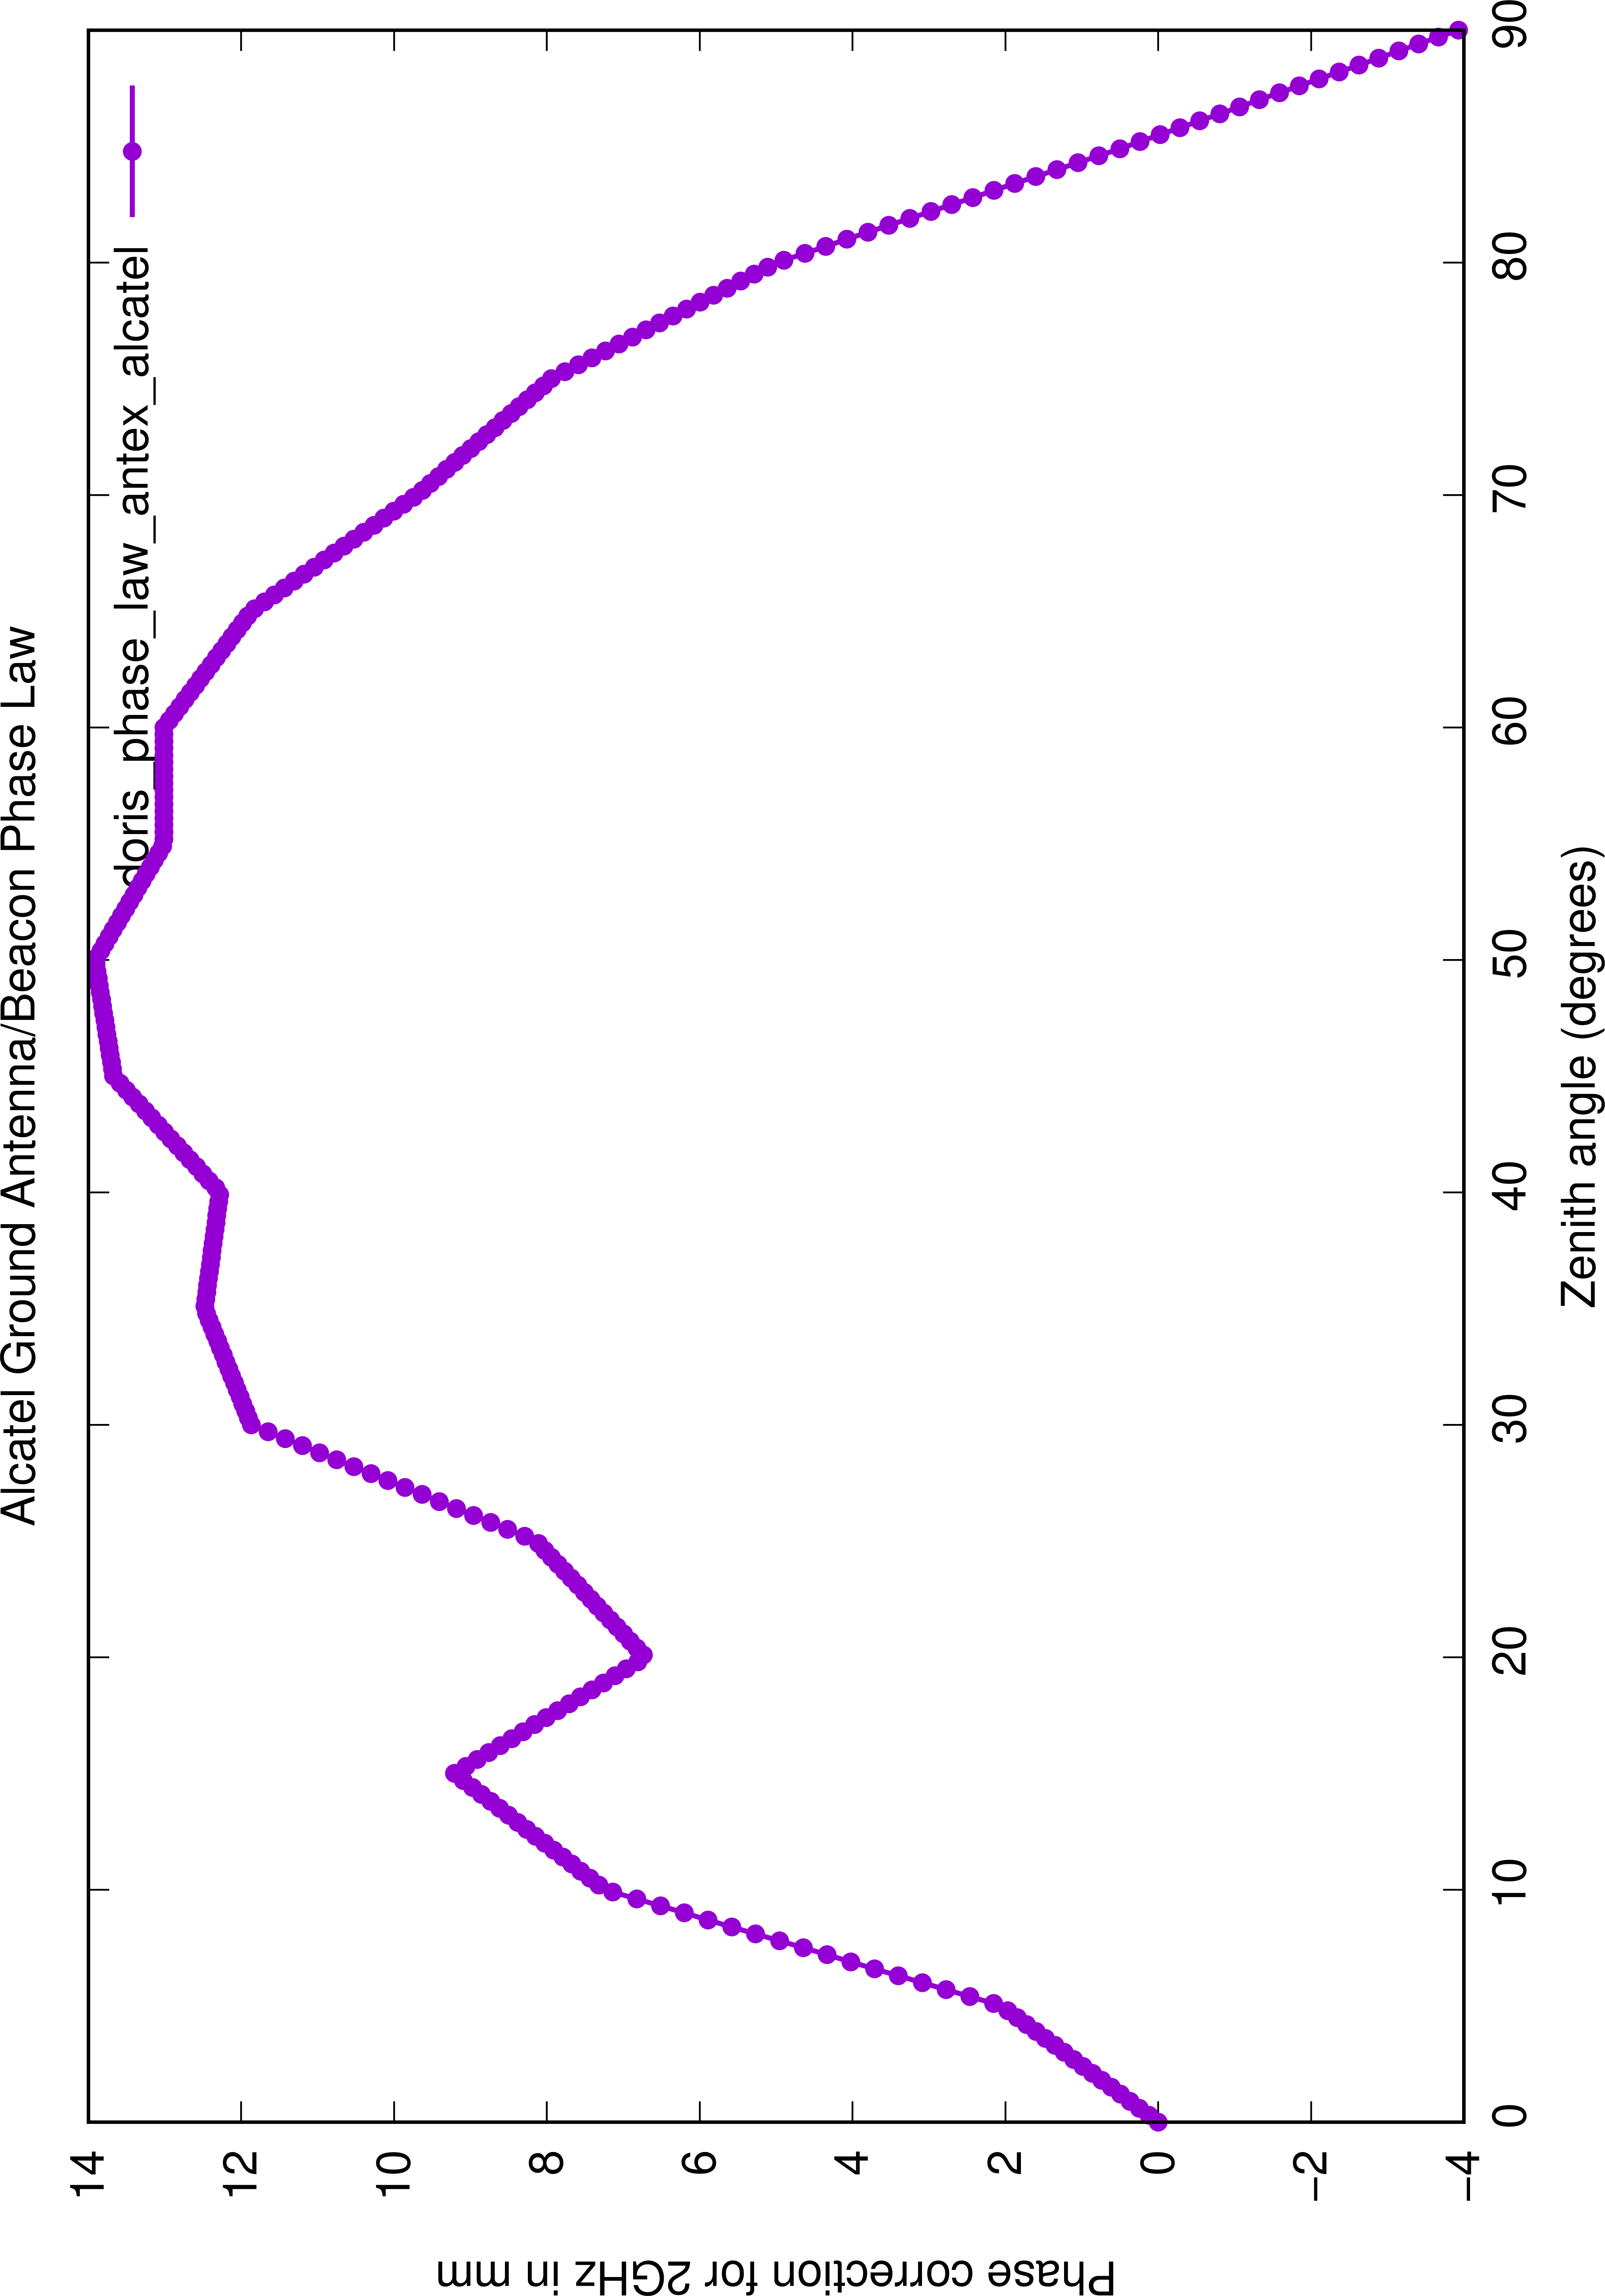
\includegraphics[width=.65\linewidth, angle=-90]{alcatel-phlaw}  
%  \caption{\scriptsize ALCATEL DORIS Ground Antenna Phase Law}
%  \label{fig:sub-first}
%\end{subfigure}
%\begin{subfigure}{0.45\textwidth}
%  \centering
%  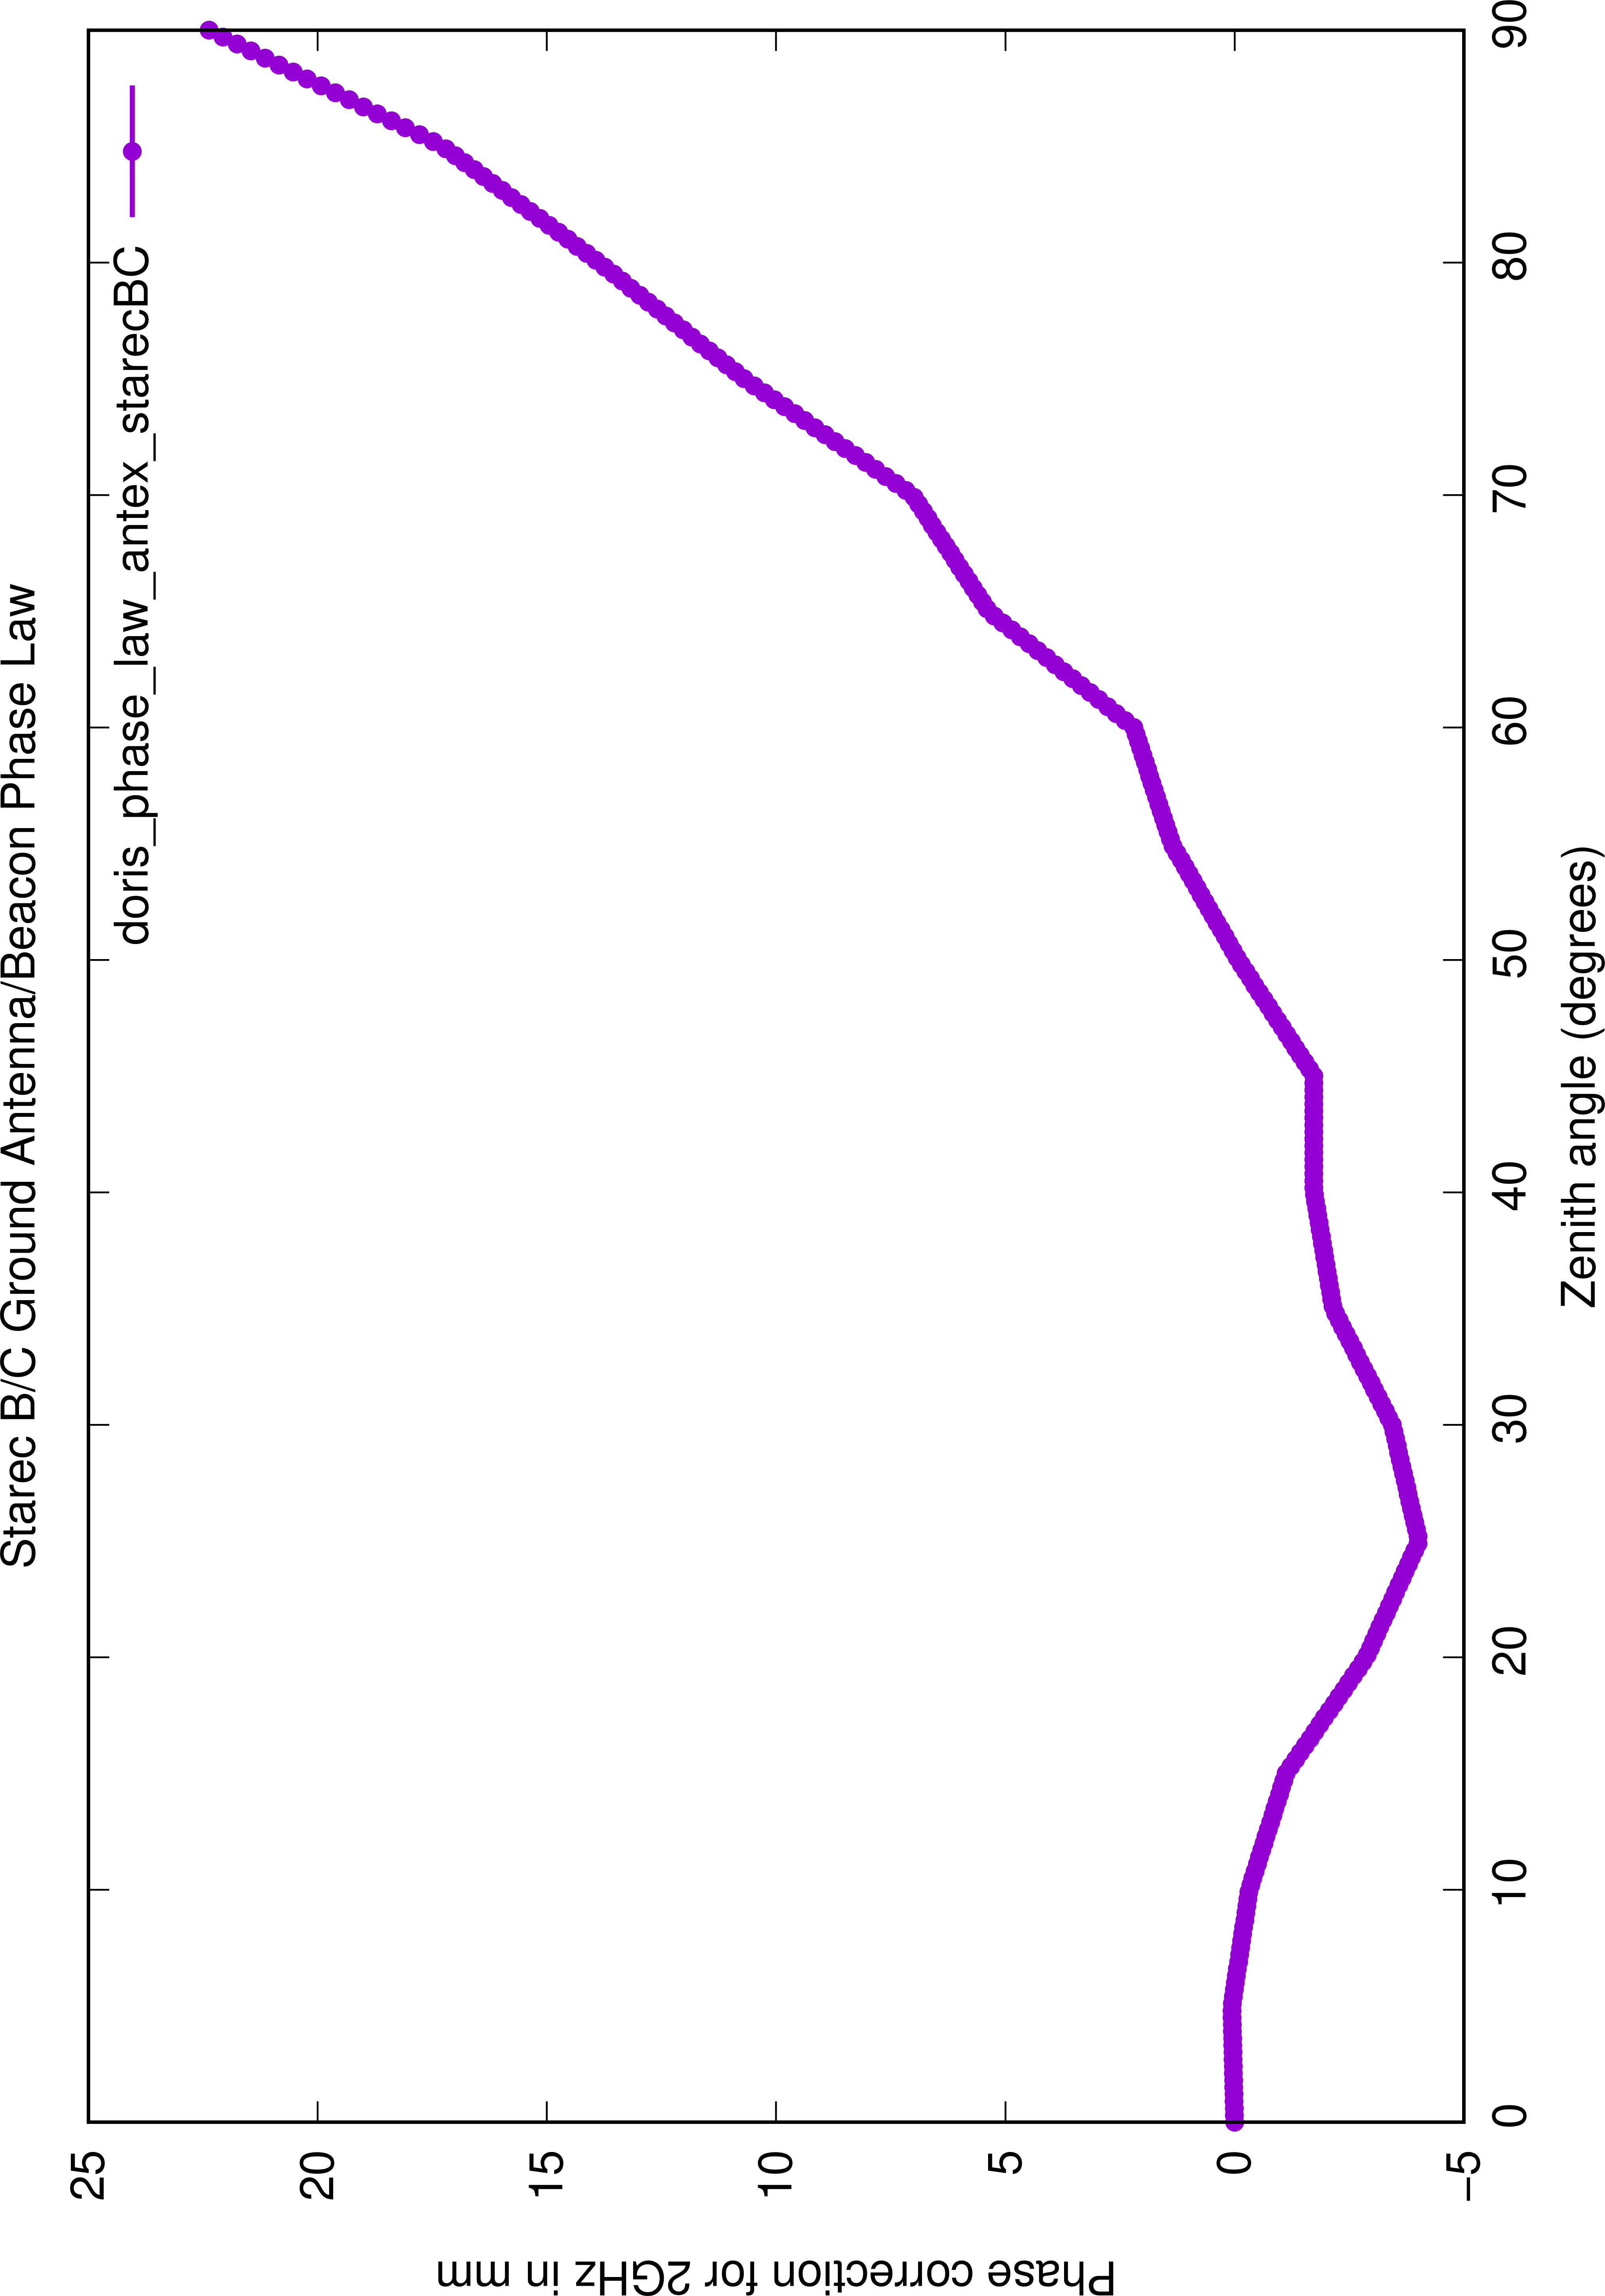
\includegraphics[width=.65\linewidth, angle=-90]{starecbc-phlaw}  
%  \caption{\scriptsize STAREC B/C DORIS Ground Antenna Phase Law}
%  \label{fig:sub-first}
%\end{subfigure}
%\caption{DORIS Ground Antenna Phase Law}
%\label{fig:ground-antenna-phase-law}
%\end{figure}